\documentclass{article}

% Russian language support
\usepackage[T2A]{fontenc}
\usepackage[russian]{babel}

% Images support
\usepackage{graphicx}

% For code listings
\usepackage{listings}

% DeclareMathOperator support
\usepackage{mathtools}

\DeclareMathOperator{\sign}{sign}
\DeclarePairedDelimiter{\abs}{\lvert}{\rvert}

\graphicspath{{../images/}}

\begin{document}
\begin{titlepage}
    \begin{center}
        \textbf{МИНИСТЕРСТВО НАУКИ И ВЫСШЕГО ОБРАЗОВАНИЯ РОССИЙСКОЙ ФЕДЕРАЦИИ}

        \textbf{
            ФЕДЕРАЛЬНОЕ ГОСУДАРСТВЕННОЕ АВТОНОМНОЕ ОБРАЗОВАТЕЛЬНОЕ УЧРЕЖДЕНИЕ
        }
        \textbf{ВЫСШЕГО ОБРАЗОВАНИЯ}

        \textbf{«БАЛТИЙСКИЙ ФЕДЕРАЛЬНЫЙ УНИВЕРСИТЕТ им. И. КАНТА»}

        \textbf{
            ИНСТИТУТ ФИЗИКО-МАТЕМАТИЧЕСКИХ НАУК И ИНФОРМАЦИОННЫХ ТЕХНОЛОГИЙ
        }

        \vspace{1.5cm}
        Выпускная квалификационная работа

        \textbf{
            Тема:
            «Численное моделирование эффекта "blow-up"
            в обратной задаче для волнового уравнения»
        }

        \textbf{Направление подготовки:}
        01.03.02: «Прикладная математика и информатика»
    \begin{flushright}
        \textbf{Выполнил:}

        Студент 4 курса

        \makebox[1in]{\hrulefill} Бока И. В.

        \textbf{Руководитель:}

        \makebox[1in]{\hrulefill} Пестов Л. Н.
    \end{flushright}

        \vfill
        Калининград

        2020
    \end{center}
\end{titlepage}

\tableofcontents

\addcontentsline{toc}{section}{Введение}
\section*{Введение}

В работе рассмотрены
численное решение задачи Коши для волнового уравнения
с использованием метода Finite-Difference Time-Domain
и
обратной задачи для волнового уравнения.

Метод Finite-Difference Time-Domain
был впервые использован
Kane Yee
для уравнений Максвелла
в его работе
\cite{numerical_solution_ibv_involving_maxwells_equations_in_isotropic_media}.


\section{Численное решение прямой задачи}

\subsection{Finite-Difference Time-Domain}

Рассмотрим задачу Коши для волнового уравнения
с однородным граничным условияем Неймана.

\begin{align*}
    \frac{\partial^2 u}{\partial t^2}
    &=
    c^2
    \left(
    \frac{\partial^2 u}{\partial x_1^2}
    + \frac{\partial^2 u}{\partial x_2^2}
    + \cdots
    + \frac{\partial^2 u}{\partial x_n^2}
    \right)
    ,
    t \in \left( 0, T \right)
    \\
    u \left( \mathbf{x}, 0 \right) &= u_0 \left( \mathbf{x} \right) \\
    \frac{\partial u}{\partial t} \left( \mathbf{x}, 0 \right) &= 0 \\
    \frac{\partial u}{\partial \mathbf{n}} \left( \mathbf{x}, t \right) &= 0
    ,
    x \in \partial \Omega
\end{align*}

Численное решение задачи можно получить
с использованием метода Finite-Difference Time-Domain
\cite{understanding_the_finite-difference_time-domain_method}.

Акустические волны есть изменения давления
\( u \left( \mathbf{x}, t \right) \).

\( c \left( \mathbf{x} \right) \)
- скорость звука в точке \( \mathbf{x} \) (не зависит от времени \( t \)).

Из физических соображений обычно рассматривают случаи \( n \le 3 \).

Рассмотрим случай \( n = 3 \).

\begin{align*}
    \frac{\partial^2 u}{\partial t^2}
    &=
    c^2
    \left(
        \frac{\partial^2 u}{\partial x^2}
        + \frac{\partial^2 u}{\partial y^2}
        + \frac{\partial^2 u}{\partial z^2}
    \right)
    ,
    t \in \left( 0, T \right)
    \\
    u \left( \mathbf{x}, 0 \right) &= u_0 \left( \mathbf{x} \right) \\
    \frac{\partial u}{\partial t} \left( \mathbf{x}, 0 \right) &= 0 \\
    \frac{\partial u}{\partial \mathbf{n}} \left( \mathbf{x} , t \right) &= 0
    ,
    x \in \partial \Omega
    \\
\end{align*}

Пусть \( \rho \left( \mathbf{x} \right) = \lim \frac{m}{V} \)
- плотность в точке \( \mathbf{x} \) (не зависит от времени \( t \)).


Пусть \( \Delta x_i = x_i - x_i^0 \).

Рассмотрим куб со стороной \( \abs{\Delta x_i} \).

Площадь поперечного сечения
\( A \left( \Delta x_i \right) = \left( \Delta x_i \right) ^2 \).

Объём \( V \left( \Delta x_i \right) = A \abs{\Delta x_i} \).

Масса \( m \left( \Delta x_i \right) \).

\setlength{\unitlength}{1cm}
\begin{picture}(8, 5)
    % Figure 1
    \put(2, 2){\line(0, 1){2}}
    \put(2, 2){\line(1, 0){2}}
    \put(2, 4){\line(1, 0){2}}
    \put(4, 2){\line(0, 1){2}}
    \put(2, 1.5){\( x_i^0 \)}
    \put(4, 1.5){\( x_i \)}
    \put(2, 3){\vector(1, 0){0.5}}
    \put(4, 3){\vector(-1, 0){0.5}}
    \put(2.2, 3.2){\( F_0 \)}
    \put(3.5, 3.2){\( F_1 \)}
    \put(1.5, 3.5){\( A \)}
    \put(4.2, 3.5){\( A \)}
    \put(0, 0){\vector(1, 0){5}}
    \put(1, 0){\circle*{0.1}}
    \put(4.5, 0.3){\( x_i \)}

    % Figure 2
    \put(8, 2){\line(0, 1){2}}
    \put(8, 2){\line(1, 0){2}}
    \put(8, 4){\line(1, 0){2}}
    \put(10, 2){\line(0, 1){2}}
    \put(8, 1.5){\( x_i \)}
    \put(10, 1.5){\( x_i^0 \)}
    \put(8, 3){\vector(1, 0){0.5}}
    \put(10, 3){\vector(-1, 0){0.5}}
    \put(8.2, 3.2){\( F_1 \)}
    \put(9.5, 3.2){\( F_0 \)}
    \put(7.5, 3.5){\( A \)}
    \put(10.2, 3.5){\( A \)}
    \put(6, 0){\vector(1, 0){5}}
    \put(7, 0){\circle*{0.1}}
    \put(10.5, 0.3){\( x_i \)}
\end{picture}

Проекция сил действующих на куб на ось \( Ox_i \): 

\begin{align*}
    F_{x_i} \left( \Delta x_i \right)
    &= \sign \left( \Delta x_i \right) \left( F_0 + F_1 \right)
    \\
    &=
    \sign \left( \Delta x_i \right)
    \left(
    u \left( \mathbf{x} \right) A
    - u \left( \mathbf{x} + \Delta x_i \mathbf{e}_i \right) A
    \right)
    \\
    &=
    \sign \left( \Delta x_i \right)
    \left(
    u \left( \mathbf{x} \right)
    - u \left( \mathbf{x} + \Delta x_i \mathbf{e}_i \right)
    \right) A
\end{align*}

где \( \mathbf{e}_i \) - базисный вектор на оси \( Ox_i \).

Второй закон Ньютона:

\begin{align*}
    \mathbf{F} &= m \mathbf{a} \\
    m \mathbf{a} &= \mathbf{F} \\
    m a_{x_i} &= F_{x_i} \\
    m \frac{\partial v_{x_i}}{\partial t}
    &=
    \sign \left( \Delta x_i \right)
    \left(
    u \left( \mathbf{x} \right)
    - u \left( \mathbf{x} + \Delta x_i \mathbf{e}_i \right)
    \right)
    A
    \\
    \frac{m}{V} \frac{\partial v{x_i}}{\partial t}
    &=
    \sign \left( \Delta x_i \right)
    \left(
    u \left( \mathbf{x} \right)
    - u \left( \mathbf{x} + \Delta x_i \mathbf{e}_i \right)
    \right)
    \frac{A}{V}
    \\
    \frac{m}{V} \frac{\partial v_{x_i}}{\partial t}
    &=
    \sign \left( \Delta x_i \right)
    \left(
    u \left( \mathbf{x} \right)
    - u \left( \mathbf{x} + \Delta x_i \mathbf{e}_i \right)
    \right)
    \frac{1}{\abs{\Delta x_i}}
    \\
    \frac{m}{V} \frac{\partial v_{x_i}}{\partial t}
    &=
    \left(
    u \left( \mathbf{x} \right)
    - u \left( \mathbf{x} + \Delta x_i \mathbf{e}_i \right)
    \right)
    \frac{\sign \left( \Delta x_i \right)}{\abs {\Delta x_i}}
    \\
    \frac{m}{V} \frac{\partial v_{x_i}}{\partial t}
    &=
    \left(
    u \left( \mathbf{x} \right)
    - u \left( \mathbf{x} + \Delta x_i \mathbf{e}_i \right)
    \right)
    \frac{1}{\sign \left( \Delta x_i \right) \abs{\Delta x_i}}
    \\
    \frac{m}{V} \frac{\partial v_{x_i}}{\partial t}
    &=
    \left(
    u \left( \mathbf{x} \right)
    - u \left( \mathbf{x} + \Delta x_i \mathbf{e}_i \right)
    \right)
    \frac{1}{\Delta x_i}
    \\
    \frac{m}{V} \frac{\partial v_{x_i}}{\partial t}
    &=
    \frac{
    \left(
    u \left( \mathbf{x} \right)
    - u \left( \mathbf{x} + \Delta x_i \mathbf{e}_i \right)
    \right)
    }
    {\Delta x_i}
    \\
    \frac{m}{V} \frac{\partial v_{x_i}}{\partial t}
    &=
    -
    \frac{
    \left(
    u \left( \mathbf{x} + \Delta x_i \mathbf{e}_i \right)
    - u \left( \mathbf{x} \right)
    \right)
    }
    {\Delta x_i}
\end{align*}

Переходя к пределу получаем
\(
\rho \frac{\partial v_{x_i}}{\partial t} = - \frac{\partial u}{\partial x_i}
\)
или
\(
\frac{\partial v_{x_i}}{\partial t}
= - \frac{1}{\rho} \frac{\partial u}{\partial x_i}
\)
.

Таким образом.

\begin{align*}
    \frac{\partial v_x}{\partial t}
    &= - \frac{1}{\rho} \frac{\partial u}{\partial x}
    \\
    \frac{\partial v_y}{\partial t}
    &= - \frac{1}{\rho} \frac{\partial u}{\partial y}
    \\
    \frac{\partial v_z}{\partial t}
    &= - \frac{1}{\rho} \frac{\partial u}{\partial z}
\end{align*}

Из уравнения состояния, при использовании нескольких приближений можно получить
\(
\frac{\partial u}{\partial t}
=
-
\rho
c^2
\left(
\frac{\partial v_x}{\partial x}
+ \frac{\partial v_y}{\partial y}
+ \frac{\partial v_z}{\partial z}
\right)
\).

Из системы уравнений

\begin{align*}
    \frac{\partial v_x}{\partial t}
    &= - \frac{1}{\rho} \frac{\partial u}{\partial x}
    \\
    \frac{\partial v_y}{\partial t}
    &= - \frac{1}{\rho} \frac{\partial u}{\partial y}
    \\
    \frac{\partial v_z}{\partial t}
    &= - \frac{1}{\rho} \frac{\partial u}{\partial z}
    \\
    \frac{\partial u}{\partial t}
    &=
    -
    \rho
    c^2
    \left(
    \frac{\partial v_x}{\partial x}
    + \frac{\partial v_y}{\partial y}
    + \frac{\partial v_z}{\partial z}
    \right)
\end{align*}

можно получить волновое уравнение:

\begin{align*}
    \frac{\partial^2 u}{\partial t^2}
    &= \frac{\partial}{\partial t} \frac{\partial u}{\partial t} \\
    &=
    \frac{\partial}{\partial t}
    \left(
    -
    \rho
    c^2
    \left(
    \frac{\partial v_x}{\partial x}
    + \frac{\partial v_y}{\partial y}
    + \frac{\partial v_z}{\partial z}
    \right)
    \right)
    \\
    &=
    - \rho c^2
    \frac{\partial}{\partial t}
    \left(
    \frac{\partial v_x}{\partial x}
    + \frac{\partial v_y}{\partial y}
    + \frac{\partial v_z}{\partial z}
    \right)
    \\
    &=
    - \rho c^2
    \left(
    \frac{\partial}{\partial t} \frac{\partial v_x}{\partial x}
    + \frac{\partial}{\partial t} \frac{\partial v_y}{\partial y}
    + \frac{\partial}{\partial t} \frac{\partial v_z}{\partial z}
    \right)
    \\
    &=
    - \rho c^2
    \left(
    \frac{\partial}{\partial x} \frac{\partial v_x}{\partial t}
    + \frac{\partial}{\partial y} \frac{\partial v_y}{\partial t}
    + \frac{\partial}{\partial z} \frac{\partial v_z}{\partial t}
    \right)
    \\
    &=
    - \rho c^2
    \left(
    \frac{\partial}{\partial x}
    \left( - \frac{1}{\rho} \frac{\partial u}{\partial x} \right)
    + \frac{\partial}{\partial y}
    \left( - \frac{1}{\rho} \frac{\partial u}{\partial y} \right)
    + \frac{\partial}{\partial z}
    \left( - \frac{1}{\rho} \frac{\partial u}{\partial z} \right)
    \right)
    \\
    &=
    - \rho c^2
    \left(
    - \frac{1}{\rho} \frac{\partial}{\partial x} \frac{\partial u}{\partial x}
    - \frac{1}{\rho} \frac{\partial}{\partial y} \frac{\partial u}{\partial y}
    - \frac{1}{\rho} \frac{\partial}{\partial z} \frac{\partial u}{\partial z}
    \right)
    \\
    &=
    \left( - \rho c^2 \right) \left( - \frac{1}{\rho} \right)
    \left(
    \frac{\partial}{\partial x} \frac{\partial u}{\partial x}
    + \frac{\partial}{\partial y} \frac{\partial u}{\partial y}
    + \frac{\partial}{\partial z} \frac{\partial u}{\partial z}
    \right)
    \\
    &=
    c^2
    \left(
    \frac{\partial^2 u}{\partial x^2}
    + \frac{\partial^2 u}{\partial y^2}
    + \frac{\partial^2 u}{\partial z^2}
    \right)
\end{align*}

Будем решать задачу численно используя метод Finite-Difference Time-Domain.
Для этого необходима дискретизация по временным и пространственным переменным.

Узел, в котором вычисляется давление,
должен быть окружён узлами, в которых вычисляются компоненты вектора скорости.
Расположение узлов отличается
от расположения
в методе Finite-Difference Time-Domain для законов Ампера и Фарадея.

Кроме того, необходимо смещение по временной переменой
- узлы, в которых вычисляется давление, должны быть смещены на полшага
от узлов, в которых вычисляются компоненты вектора скорости.

Будем считать пространственный шаг одинаковым \( h_x = h_y = h_z = h \).

Заменим производные конечными разностями.

\begin{align*}
    u^l \left[ i, j, k \right]
    &\approx u \left( ih, jh, kh, l \Delta_t \right)
    \\
    v_x^{l + \frac{1}{2}} \left[ i, j, k \right]
    & \approx
    v_x
    \left(
    \left( i + \frac{1}{2} \right) h,
    jh,
    kh,
    \left( l + \frac{1}{2} \right) \Delta_t
    \right)
    \\
    v_y^{l + \frac{1}{2}} \left[ i, j, k \right]
    & \approx
    v_y
    \left(
    ih,
    \left( j + \frac{1}{2} \right) h,
    kh,
    \left( l + \frac{1}{2} \right) \Delta_t
    \right)
    \\
    v_z^{l + \frac{1}{2}} \left[ i, j, k \right]
    & \approx
    v_z
    \left(
    ih,
    jh,
    \left( k + \frac{1}{2} \right) h,
    \left( l + \frac{1}{2} \right) \Delta_t
    \right)
    \\
    u^l \left[ i, j, k \right]
    &= 
    u^{l-1} \left[ i, j, k \right]
    -
    \frac{\Delta_t \rho c^2}{h}
    \left( \right.
    \\
    &v_x^{l - \frac{1}{2}} \left[ i, j, k \right]
    - v_x^{l - \frac{1}{2}} \left[ i - 1, j, k \right]
    \\
    &+ v_y^{l - \frac{1}{2}} \left[ i, j, k \right]
    - v_y^{l - \frac{1}{2}} \left[ i, j - 1, k \right]
    \\
    &+ v_z^{l - \frac{1}{2}} \left[ i, j, k \right]
    - v_z^{l - \frac{1}{2}} \left[ i, j, k - 1 \right]
    \left. \right)
    \\
    v_x^{l + \frac{1}{2}} \left[ i, j, k \right]
    &=
    v_x^{l - \frac{1}{2}} \left[ i, j, k \right]
    -
    \frac{\Delta_t}{h \rho}
    \left( u^l \left[ i + 1, j, k \right] - u^l \left[ i, j, k \right] \right)
    \\
    v_y^{l + \frac{1}{2}} \left[ i, j, k \right]
    &=
    v_y^{l - \frac{1}{2}} \left[ i, j, k \right]
    -
    \frac{\Delta_t}{h \rho}
    \left( u^l \left[ i, j + 1, k \right] - u^l \left[ i, j, k \right] \right)
    \\
    v_z^{l + \frac{1}{2}} \left[ i, j, k \right]
    &=
    v_z^{l - \frac{1}{2}} \left[ i, j, k \right]
    -
    \frac{\Delta_t}{h \rho}
    \left( u^l \left[ i, j, k + 1 \right] - u^l \left[ i, j, k \right] \right)
    \\
\end{align*}

Шаг по времени нужно выбирать так, чтобы число Куранта не превосходило единицу.

\begin{align*}
    C = \frac{\sup \left( c \right) \Delta_t}{h} \\
    C \le 1 \\
    \frac{\sup \left( c \right) \Delta_t}{h} \le 1 \\
    \Delta_t \le \frac{h}{\sup \left( c \right)}
\end{align*}

Для простоты в дальнейшем будем рассматривать случай \( n = 2 \):

\begin{align*}
    \frac{\partial v_x}{\partial t}
    &= - \frac{1}{\rho} \frac{\partial u}{\partial x}
    \\
    \frac{\partial v_y}{\partial t}
    &= - \frac{1}{\rho} \frac{\partial u}{\partial y}
    \\
    \frac{\partial u}{\partial t}
    &=
    -
    \rho
    c^2
    \left(
    \frac{\partial v_x}{\partial x} + \frac{\partial v_y}{\partial y}
    \right)
\end{align*}

\begin{align*}
    u^l \left[ i, j \right] & \approx u \left( ih, jh, l \Delta_t \right) \\
    v_x^{l + \frac{1}{2}} \left[ i, j \right]
    & \approx
    v_x
    \left(
    \left( i + \frac{1}{2} \right) h,
    jh,
    \left( l + \frac{1}{2} \right) \Delta_t
    \right)
    \\
    v_y^{l + \frac{1}{2}} \left[ i, j \right]
    & \approx
    v_y
    \left(
    ih,
    \left( j + \frac{1}{2} \right) h,
    \left( l + \frac{1}{2} \right) \Delta_t
    \right)
    \\
    u^l \left[ i, j \right]
    &= 
    u^{l-1} \left[ i, j \right]
    -
    \frac{\Delta_t \rho c^2}{h}
    \left( \right.
    \\
    &v_x^{l - \frac{1}{2}} \left[ i, j \right]
    - v_x^{l - \frac{1}{2}} \left[ i - 1, j \right]
    + v_y^{l - \frac{1}{2}} \left[ i, j \right]
    - v_y^{l - \frac{1}{2}} \left[ i, j - 1 \right]
    \left. \right)
    \\
    v_x^{l + \frac{1}{2}} \left[ i, j \right]
    &=
    v_x^{l - \frac{1}{2}} \left[ i, j \right]
    -
    \frac{\Delta_t}{h \rho}
    \left( u^l \left[ i + 1, j \right] - u^l \left[ i, j \right] \right) \\
    v_y^{l + \frac{1}{2}} \left[ i, j \right]
    &=
    v_y^{l - \frac{1}{2}} \left[ i, j \right]
    -
    \frac{\Delta_t}{h \rho}
    \left( u^l \left[ i, j + 1 \right] - u^l \left[ i, j \right] \right) \\
\end{align*}

Заменим аппроксимацию производной по пространственным переменным
на центральную аппроксимацию 12-того порядка.
Формулы не приводятся по причине их громоздкости.

\begin{figure}
    \caption{Начальные условия}
\noindent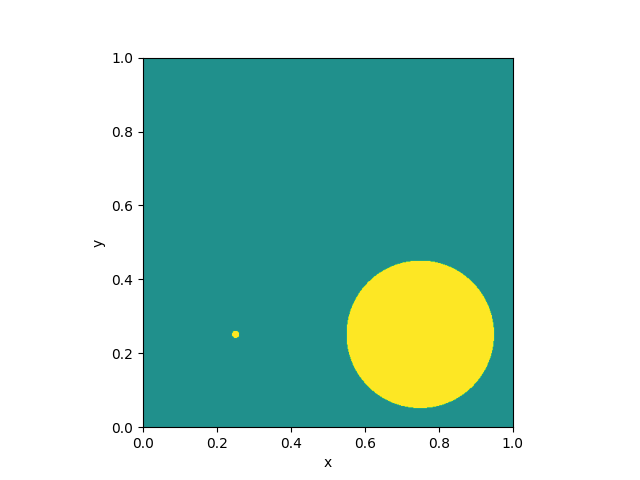
\includegraphics[width=\textwidth]{initial}
\end{figure}

\begin{figure}
    \caption{Решение прямой задачи с однородным граничным условием Неймана}
\noindent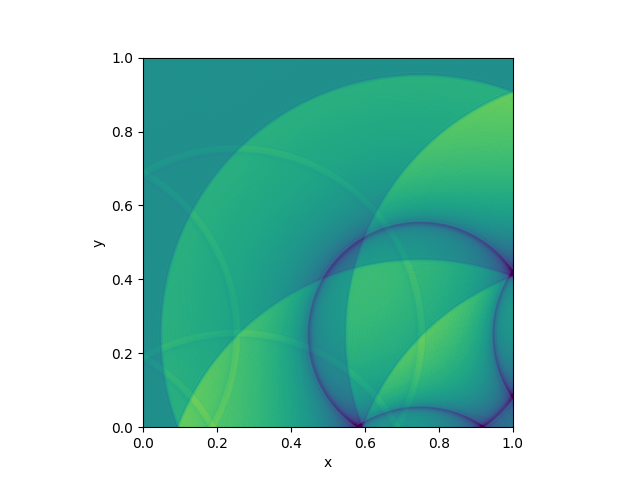
\includegraphics[width=\textwidth]{forward_neyman_zero_boundary}
\end{figure}


\subsection{Perfecty Mathed Layer}

На практике бывает необходимо решить задачу для неограниченной области.
Для этого можно увеличить область \( \Omega \) настолько,
что за время \( T \) волны не дойдут до границы \( \partial \Omega \).
Однако, такой способ неудобен, так как требует больших вычислительных ресурсов.
Поэтому на практике используют поглащающие слои на границе,
которые позволяют избежать отражения волн.

Техника Perfectly Matched Layer была впервые сформулирована
в работе Jean-Pierre Berenger'а
\cite{a_perfectly_matched_layer_for_the_absorption_of_electromagnetic_waves}.
Изначально Perfectly Matched Layer использовался для уравнений Максвелла.
 

Вместо системы уравнений рассмотренной в предыдущем подразделе
рассмотрим следующую систему уравнений:

\begin{align*}
    \frac{\partial v_x}{\partial t} + \sigma_x v_x
    &= - \frac{1}{\rho} \frac{\partial \left( u_x + u_y \right) }{\partial x}
    \\
    \frac{\partial v_y}{\partial t} + \sigma_y v_y
    &= - \frac{1}{\rho} \frac{\partial \left( u_x + u_y \right) }{\partial y}
    \\
    \frac{\partial u_x}{\partial t} + \sigma_x^* u_x
    &= - \rho c^2 \frac{\partial v_x}{\partial x}
    \\
    \frac{\partial u_y}{\partial t} + \sigma_y^* u_y
    &= - \rho c^2 \frac{\partial v_x}{\partial x}
\end{align*}

Заметим, что при \( \sigma_x = \sigma_x^* = \sigma_y = \sigma_y^* = 0 \)
получим систему уравнений эквивалентную волновому уравнению.

Во внутренней области положим
\( \sigma_x = \sigma_x^* = \sigma_y = \sigma_y^* = 0 \).

При значениях \( x \) близких к граничным
\( \sigma_x > 0 \) и \( \sigma_x^* > 0 \).
При значениях \( y \) близких к граничным
\( \sigma_y > 0 \) и \( \sigma_y^* > 0 \).
Причём значение функций \( \sigma \) монотонно возрастает
от нуля до максимума по мере приближения к границе.

\begin{figure}
    \caption{Решение прямой задачи с Perfect Matched Layer на границе}
\noindent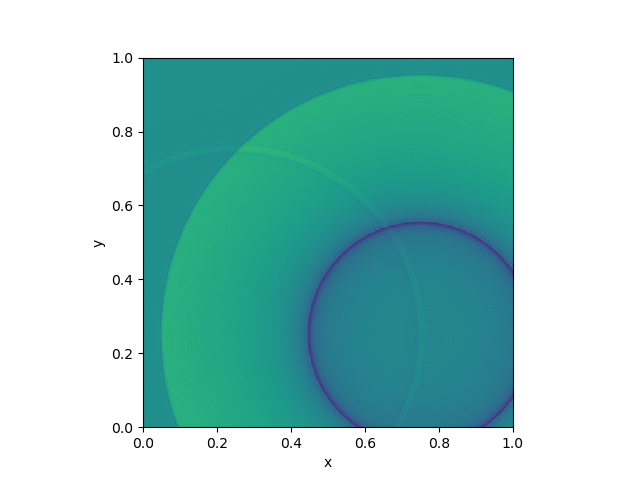
\includegraphics[width=\textwidth]{forward_perfect_matched_layer}
\end{figure}

\begin{figure}
    \caption{Решение прямой задачи с Perfect Matched Layer на границе - переменная скорость}
\noindent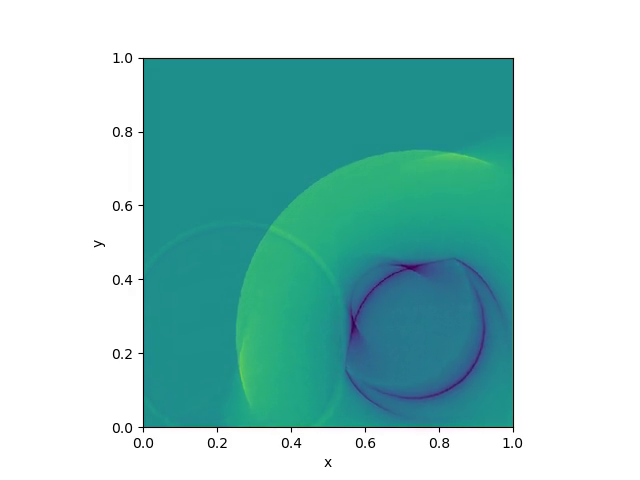
\includegraphics[width=\textwidth]{forward_perfect_matched_layer_variable_speed}
\end{figure}



\section{Обратная задача}

\subsection{Метод граничного управления}

Рассмотрим обратную задачу для волнового уравнения.

\begin{align*}
    \frac{\partial^2 u}{\partial t^2}
    &=
    c^2
    \left(
    \frac{\partial^2 u}{\partial x_1^2}
    + \frac{\partial^2 u}{\partial x_2^2}
    + \cdots
    + \frac{\partial^2 u}{\partial x_n^2}
    \right)
    ,
    t \in \left( 0, T \right)
    \\
    u \left( \mathbf{x}, 0 \right) &= 0 \\
    \frac{\partial u}{\partial t} \left( \mathbf{x}, 0 \right) &= 0 \\
    u \left( \mathbf{x}, t \right)
    &=
    \phi \left( \mathbf{x}, t \right),
    t \ \in \left( 0, T \right), x \in \partial \Omega
    \\
    \frac{\partial u}{\partial \mathbf{n}} \left( \mathbf{x}, t \right)
    &=
    f \left( \mathbf{x} \right)
    ,
    x \in \partial \Omega
\end{align*}

Обратная задача граничного управления состоит в
отыскании функции \( f \left( \mathbf{x} \right) \),
зная функию \( \phi \left( \mathbf{x} \right) \).


\subsection{Эффект blow-up}



\addcontentsline{toc}{section}{Заключение}
\section*{Заключение}

Было рассмотрено решение прямой и обратной задачи для волнового уравнения.


\addcontentsline{toc}{section}{Приложения}
\section*{Приложения}

Программа на языке программирования Python
для решения прямой задачи методом Finite-Difference Time-Domain
с граничным условием Неймана:
\lstinputlisting[language=Python,breaklines]
{../programs/src/solve_neyman_zero_boundary.py}

Программа на языке программирования Python
для решения прямой задачи методом Finite-Difference Time-Domain
с использованием техники Perfect Matched Layer:
\lstinputlisting[language=Python,breaklines]
{../programs/src/solve_perfect_matched_layer.py}

Программа на языке программирования Python
для решения прямой задачи методом Finite-Difference Time-Domain
с использованием техники Perfect Matched Layer - переменная скорость:
\lstinputlisting[language=Python,breaklines]
{../programs/src/solve_perfect_matched_layer_variable_speed.py}


\addcontentsline{toc}{section}{Список литературы}
\bibliographystyle{unsrt}
\bibliography{bibliography}


\end{document}
